\documentclass[11pt,letterpaper]{article}
\usepackage[top=3cm, bottom=2cm, left=2cm, right=2cm, columnsep=20pt]{geometry}
\usepackage{pdfpages}
\usepackage{graphicx}
\usepackage{etoolbox}
\apptocmd{\sloppy}{\hbadness 10000\relax}{}{}
% \usepackage[numbers]{natbib}
\usepackage[T1]{fontenc}
\usepackage{ragged2e}
\usepackage[french]{babel}
\usepackage{listings}
\usepackage{color}
\usepackage{soul}
\usepackage[utf8]{inputenc}
\usepackage[export]{adjustbox}
\usepackage{caption}
\usepackage{amsmath}
\usepackage{amssymb}
\usepackage{float}
\usepackage{csquotes}
\usepackage{fancyhdr}
\usepackage{wallpaper}
\usepackage{siunitx}
\usepackage[indent]{parskip}
\usepackage{textcomp}
\usepackage{gensymb}
\usepackage{multirow}
\usepackage[hidelinks]{hyperref}
\usepackage{abstract}
\renewcommand{\abstractnamefont}{\normalfont\bfseries}
\renewcommand{\abstracttextfont}{\normalfont\itshape}
\usepackage{titlesec}
\titleformat{\section}{\large\bfseries}{\thesection}{1em}{}
\titleformat{\subsection}{\normalsize\bfseries}{\thesubsection}{1em}{}
\titleformat{\subsubsection}{\normalsize\bfseries}{\thesubsubsection}{1em}{}

\usepackage{xcolor}
\definecolor{codegreen}{rgb}{0,0.6,0}
\definecolor{codegray}{rgb}{0.5,0.5,0.5}
\definecolor{codepurple}{rgb}{0.58,0,0.82}
\definecolor{backcolour}{rgb}{0.95,0.95,0.92}
\lstdefinestyle{mystyle}{
    backgroundcolor=\color{backcolour},   
    commentstyle=\color{codegreen},
    keywordstyle=\color{magenta},
    numberstyle=\tiny\color{codegray},
    stringstyle=\color{codepurple},
    basicstyle=\ttfamily\footnotesize,
    breakatwhitespace=false,         
    breaklines=true,                 
    captionpos=b,                    
    keepspaces=true,                 
    numbers=left,                    
    numbersep=5pt,                  
    showspaces=false,                
    showstringspaces=false,
    showtabs=false,                  
    tabsize=2
}
\lstset{style=mystyle}

\usepackage[most]{tcolorbox}
\newtcolorbox{note}[1][]{
  enhanced jigsaw,
  borderline west={2pt}{0pt}{black},
  sharp corners,
  boxrule=0pt, 
  fonttitle={\large\bfseries},
  coltitle={black},
  title={Note:\ },
  attach title to upper,
  #1
}

%----------------------------------------------------

\setlength{\parindent}{0pt}
\DeclareCaptionLabelFormat{mycaptionlabel}{#1 #2}
\captionsetup[figure]{labelsep=colon}
\captionsetup{labelformat=mycaptionlabel}
\captionsetup[figure]{name={Figure }}
\newcommand{\inlinecode}{\normalfont\texttt}
\usepackage{enumitem}
\setlist[itemize]{label=\textbullet}

\begin{document}
\begin{titlepage}
\center

\begin{figure}
    \ThisULCornerWallPaper{.4}{Polytechnique_signature-RGB-gauche_FR.png}
\end{figure}
\vspace*{2 cm}

\textsc{\Large \textbf{PHS2223 --} Introduction à l'optique moderne}\\[0.5cm]
\large{\textbf{Équipe : 04}}\\[1.5cm]

\rule{\linewidth}{0.5mm} \\[0.5cm]
\Large{\textbf{Expérience 1}} \\[0.2cm]
\text{Microscopie confocale}\\
\rule{\linewidth}{0.2mm} \\[2.3cm]

\large{\textbf{Présenté à}\\
  Guillaume Sheehy\\
  Esmat Zamani\\[2.5cm]
  \textbf{Par :}\\
  Émile \textbf{Guertin-Picard} (2208363)\\
  Laura-Li \textbf{Gilbert} (2204234)\\
  Tom \textbf{Dessauvages} (2133573)\\[3cm]}

\large{\today\\
Département de Génie Physique\\
Polytechnique Montréal\\}

\end{titlepage}

%----------------------------------------------------

\tableofcontents
\pagenumbering{roman}
\newpage

\pagestyle{fancy}
\setlength{\headheight}{14pt}
\renewcommand{\headrulewidth}{0pt}
\fancyfoot[R]{\thepage}

\pagestyle{fancy}
\fancyhf{}
\renewcommand{\headrulewidth}{1pt}
\fancyhead[L]{\textbf{PHS2223}}
\fancyhead[C]{titre}
\fancyhead[R]{date}
\fancyfoot[R]{\thepage}

\pagenumbering{arabic}
\setcounter{page}{1}

%----------------------------------------------------

\section{Résultats}

\subsection{Estimation de la résolution}

Les figures \ref{brutes 1} et \ref{brutes 2} présentent sous la forme de graphiques, les données brutes recueillies lors du laboratoire. 

% Résultats brut 
\begin{figure}[h!]
    \centering
    \begin{minipage}[t]{0.46\linewidth}
        \centering
        \includegraphics[scale=0.32]{Données brutes 1.png}
        \caption{Données brutes obtenues pour le système avec pinhole}
        \label{brutes 1}
    \end{minipage}\hfill
    \begin{minipage}[t]{0.5\linewidth}
        \centering
        \includegraphics[scale=0.32]{Données brutes 2.png}
        \caption{Données brutes obtenues pour le système sans pinhole}
        \label{brutes 2}
    \end{minipage}

\end{figure}

Au regard de l'allure de ces données, la fonction utilisées pour en faire un fit est une somme de fonctions gaussiennes centrées selon les positions des différents maximums d'amplitude. L'utilisation de la librairie \textit{lm.fit} de python permet de déterminer les valeurs optimales de ces courbes de tendances et de les représenter. Les figures \ref{fit 1} et \ref{fit 2} présentent sous la forme de graphiques, les fonctions de fitting obtenues pour les deux jeux de données brutes différents. 

\begin{figure}[h!]
    \centering
    \begin{minipage}[t]{0.46\linewidth}
        \centering
        \includegraphics[scale=0.32]{Données fit 1.png}
        \caption{Partie réelle et imaginaire du signal brut pour 10ms}
        \label{fit 1}
    \end{minipage}\hfill
    \begin{minipage}[t]{0.5\linewidth}
        \centering
        \includegraphics[scale=0.32]{Données fit 2.png}
        \caption{Phase du signal brut pour 10ms}
        \label{fit 2}
    \end{minipage}
\end{figure}

Ces représentations du signal sous la forme de somme de courbes gaussiennes permettent de mettre en évidence deux maximums d'amplitudes pour chacune des séries de données. L'amplitude représentative de la résolution du système est celle de valeur maximale. Cette résolution, représentée comme étant la largeur de la courbe à mi-hauteur de l'amplitude maximale peut, elle aussi être estimée à l'aide de \textit{lm.fit}. Le tableau \ref{FMWH} représente les résolutions obtenues ainsi que les erreurs qui leurs sont associées en fonction de la série de données :

\begin{table}[H]
\centering
\begin{tabular}{|p{3.2cm}|p{4.2cm}|p{3.2cm}|}
\cline{2-3}
\multicolumn{1}{c|}{} & \textbf{Largeur à mi-hauteur} & \textbf{Erreur} \\
\hline
\textbf{Avec pinhole} & 1.317578 & 0.092557 \\
\hline
\textbf{Sans pinhole} & 5.742349 & 0.943043 \\
\hline
\end{tabular}
\caption{Largeur à mi-hauteur et erreurs en fonction du jeu de données}
\label{FMWH}
\end{table}

\subsection{Analyse de données de LSCM en fluorescence}

Une image 3D acquise en microscopie confocale par un microscope \textit{Leica TCS SP5 MP} est analysée. Les données
acquises au préalable sont des cellules de prostate \textit{RWPE-1}, avec plusieurs cellules de cancer de la prostate
\textit{PC3} présentes. La figure \ref{non_yes_confo} présente côte à côte une image de ces cellules pour comparer
l'image d'un système non-confocal à l'image d'un système confocal.

\begin{figure}[H]
  \centering
  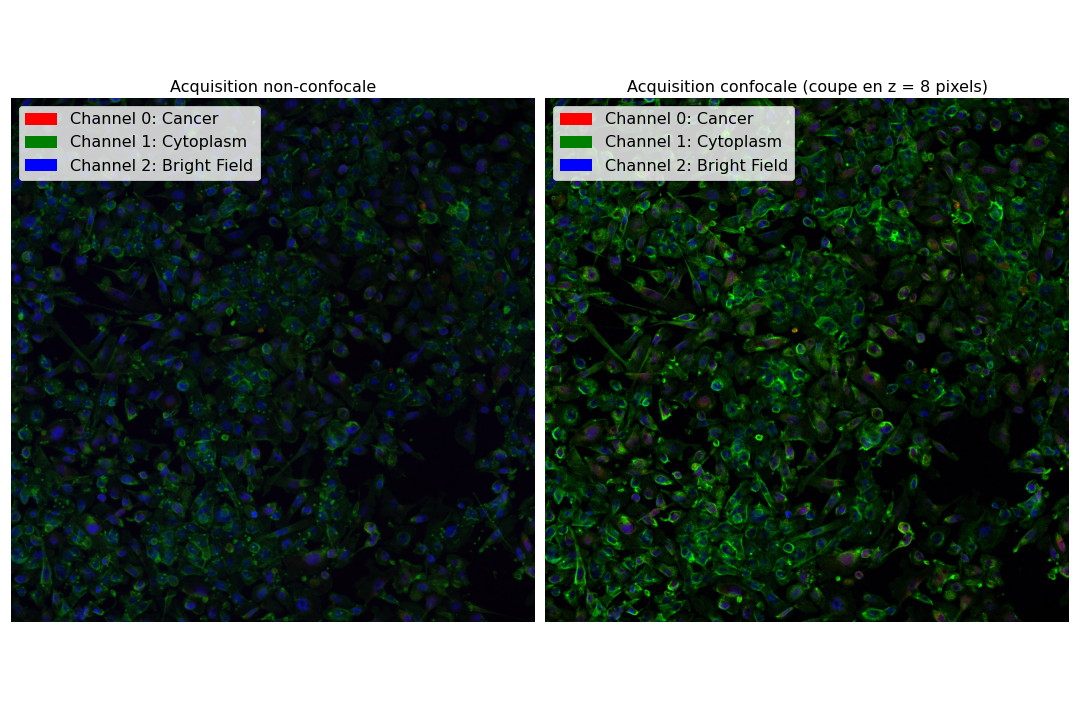
\includegraphics[scale=0.45]{non_and_yes_confocal.png}
  \caption{Comparaison de l'imagerie obtenue d'un système non-confocal (à gauche) à celle d'un système confocal (à droite).}
  \label{non_yes_confo}
\end{figure}

Il est possible de voir une meilleure résolution sur l'acquisition confocale, ce qui résulte en des contours plus définis.
Ensuite, la figure \ref{3d_cells} présente trois coupes de l'image 3D autour du même point dants l'espace afin de
représenter le volume de quelques cellules.

\begin{figure}[H]
  \centering
  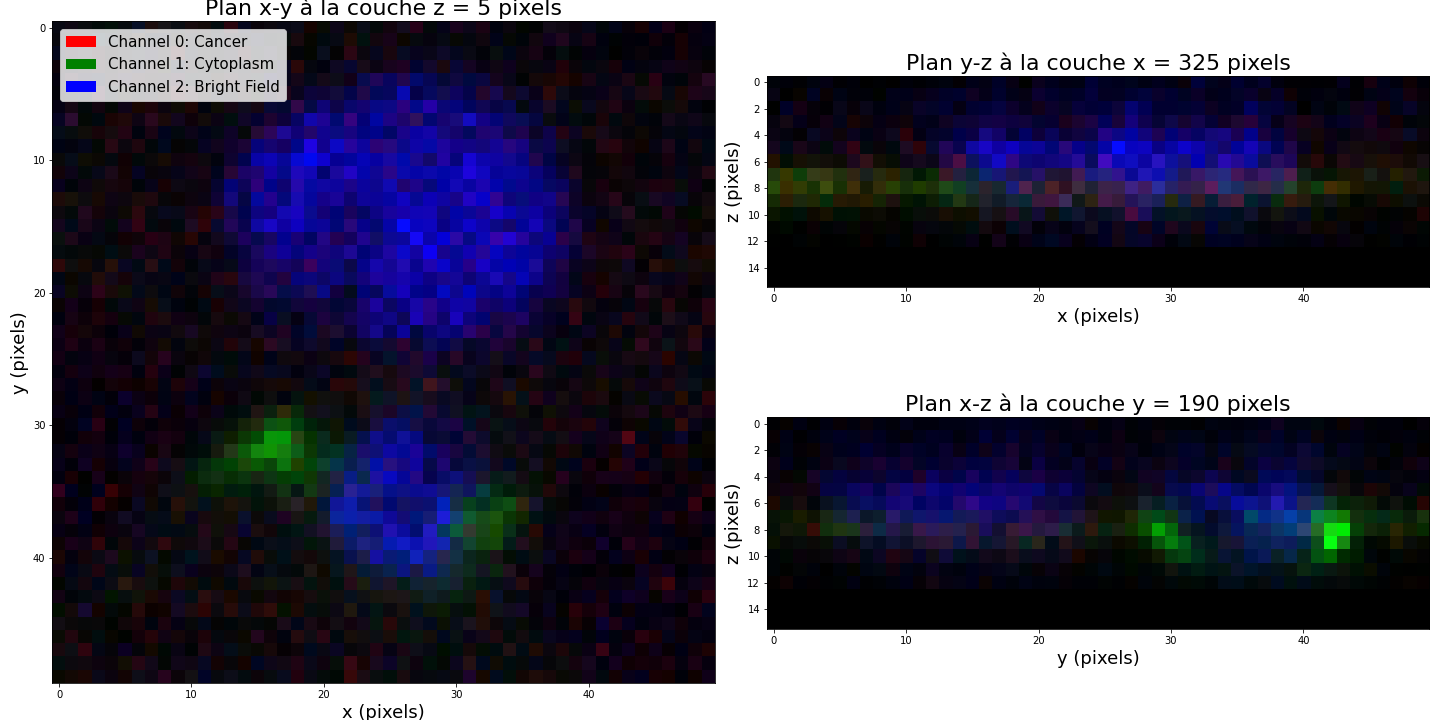
\includegraphics[scale=0.34]{volume.png}
  \caption{Volume de deux cellules bien visibles par LSCM en fluorescence présenté en trois plans.}
  \label{3d_cells}
\end{figure}


\section{Discussion}

\subsection{Retour sur l'hypothèse}

%TODO : comparaision mesure axiale entre hypothese et expérience

\subsection{Analyse des causes d'erreurs}

%TODO

vieux laser avec deux pics d'intensité
mauvais alignement de base (surtout l'alignement des back reflections)
désalignement au fur et à mesure des manipulations
incertitudes (surtout sur le power meter)

\subsection{Question 1}

%TODO

(de ce que j'ai compris apres avoir jasé avec Noémie lol)
tu peux tag certaines parties d'organismes vivants avec des fluorophores.
les couleurs viennent de ces différents fluorophores
un canal analyse qu'un type de fluorophore

\subsection{Question 2}

%TODO : trouver la source, puis confirmer apres que ça fit avec l'image 3d

\subsection{Question 3}

%TODO

le pinhole améliore la netteté des images, la définition des cellules, etc.
perte de puissance avec un pinhole, un trop petit bloquerait toute image
voir sources pour le shit de plus petit sténopé possible  

\subsection{Question 4}

%TODO

faire reference a la figure prostate side by side

\section{Conclusion}

%TODO

\begin{lstlisting}[language=python]
print("l'exam d'optique etait deg")
\end{lstlisting}



\clearpage

%TODO
% \bibliographystyle{unsrtnat}
% \bibliography{My_Library}

\end{document}
